\section{Introduction}
\label{sec:introduction}

The emergence of low power wireless systems in past decades was followed by attempts at optimizing energy efficiency and power consumption to facilitate long lifetime sensing deployments.  
%Research in this area was marked by many successes in the form of efficient time synchronization algorithms, routing protocols, new sensing paradigms, and the emergence of several widely-adopted operating systems for embedded systems (e.g., [\citeNP{tinyos}; \citeNP{contiki}]).
 In recent years, newer integrated circuit fabrication technologies have introduced several additional variables into the energy management game; as feature sizes continue to shrink, power variation on a per-instance level has become a non-trivial factor [\citeNP{Borkar:2003}; \citeNP{gupta2003}]. 

%Figure \ref{fig:variation} offers more intuition into the matter, showing the projected variation in idle and overall power as projected by the International Technology Roadmap for Semiconductors (ITRS) for years to come \cite{ITRS} as well as recent variability results in the literature. 

%\begin{figure}
%\centering
%\includegraphics[width=0.5\textwidth]{figures/projected_variations}
%\caption{\label{fig:variation}ITRS projections for sleep and idle power variability with measurements from recent %literature.}
%\end{figure}

Per-instance power variations are particularly exaggerated for idle power consumption, motivating the need to mitigate the effects of variability in systems whose operation is dominated by long idle states.  Figure \ref{fig:itrs} provides more insight into the matter: the International Technology Roadmap for Semiconductors (ITRS) predicts as much as 600\% variation in static (idle) power and over 100\% in total power by the year 2022 \cite{ITRS}. One domain that stands to benefit from research into combatting hardware variation is that of low power embedded systems and low power sensors, where the application is often that of sensing, routing, or processing data.  

In systems where computation is severely constrained by anemic energy reserves and where a long overall system lifetime is desired, maximizing the utility of a given application subject to these constraints is both challenging and an important step towards achieving high quality deployments.  Currently, developers assume some power consumption model prior to deployment, and this can have several undesired effects.  Underestimation of system power consumption can lead to a reduction in lifetime which will eventually impact quality of service, while guardbanding against worst-case power consumption by using overly conservative estimates can reduce application quality for the entirety of the lifetime. The potential solution space is shown in Figure \ref{fig:qualityandlifetime}, where the optimal solution is one that maximizes quality without decreasing lifetime. Furthermore, the distribution of power in systems comprised of multiple heterogeneous tasks is oftentimes fixed in software prior to deployment as well, placing the burden of optimizing energy usage on developers who may remain oblivious to variations in power consumption altogether. 

%Considerable research has focused on exposing energy and power measurements or estimates to the developer and even to the end user.  For example, techniques using linear combinations of instruction and performance counters [\citeNP{sun2012}; \citeNP{singh2009}], activity monitoring strategies \cite{appscope}, and various battery discharge-based models \cite{zhang2010} have been explored as tools for providing system-wide, application-specific, and even per-process granularities of energy usage.  Improved techniques for accurately  estimating and measuring power consumption will enable online power management in ways that were infeasible before, helping mitigate fabrication-induced per-instance chip variation as well.

Perhaps the most widely used and most effective strategies for extending the lifetime of energy-constrained systems are those based on controlling the ratio of system active time to total system time, or \emph{duty cycling} a system.  Duty cycled systems take advantage of the disparity between active and idle power consumption, greatly increasing the lifetime of systems where latency and throughput constraints can be relaxed. Because of temperature and instance dependencies in power consumption, however, arriving at an optimal system-wide duty cycle ratio to achieve a lifetime goal given an energy constraint is difficult to do without \emph{a priori} knowledge of instance-specific power models and temperature statistics for the target deployment location \cite{Wanner:2012}. Furthermore, applications involving more than one task necessitate notions of fairness and utility---specifically, how should active processor time be distributed between each task so as to maximize the utility of the application and still meet the desired lifetime goal?

\begin{figure*}[t]
\centering
{\centering
\begin{minipage}{0.47\textwidth}
  \centering
\includegraphics[width=\textwidth]{figures/itrs}
  \captionof{figure}{\label{fig:itrs}ITRS predictions for processor power variation for years to come}
\end{minipage}
\hspace{.04\textwidth}
\begin{minipage}{0.47\textwidth}
  \centering
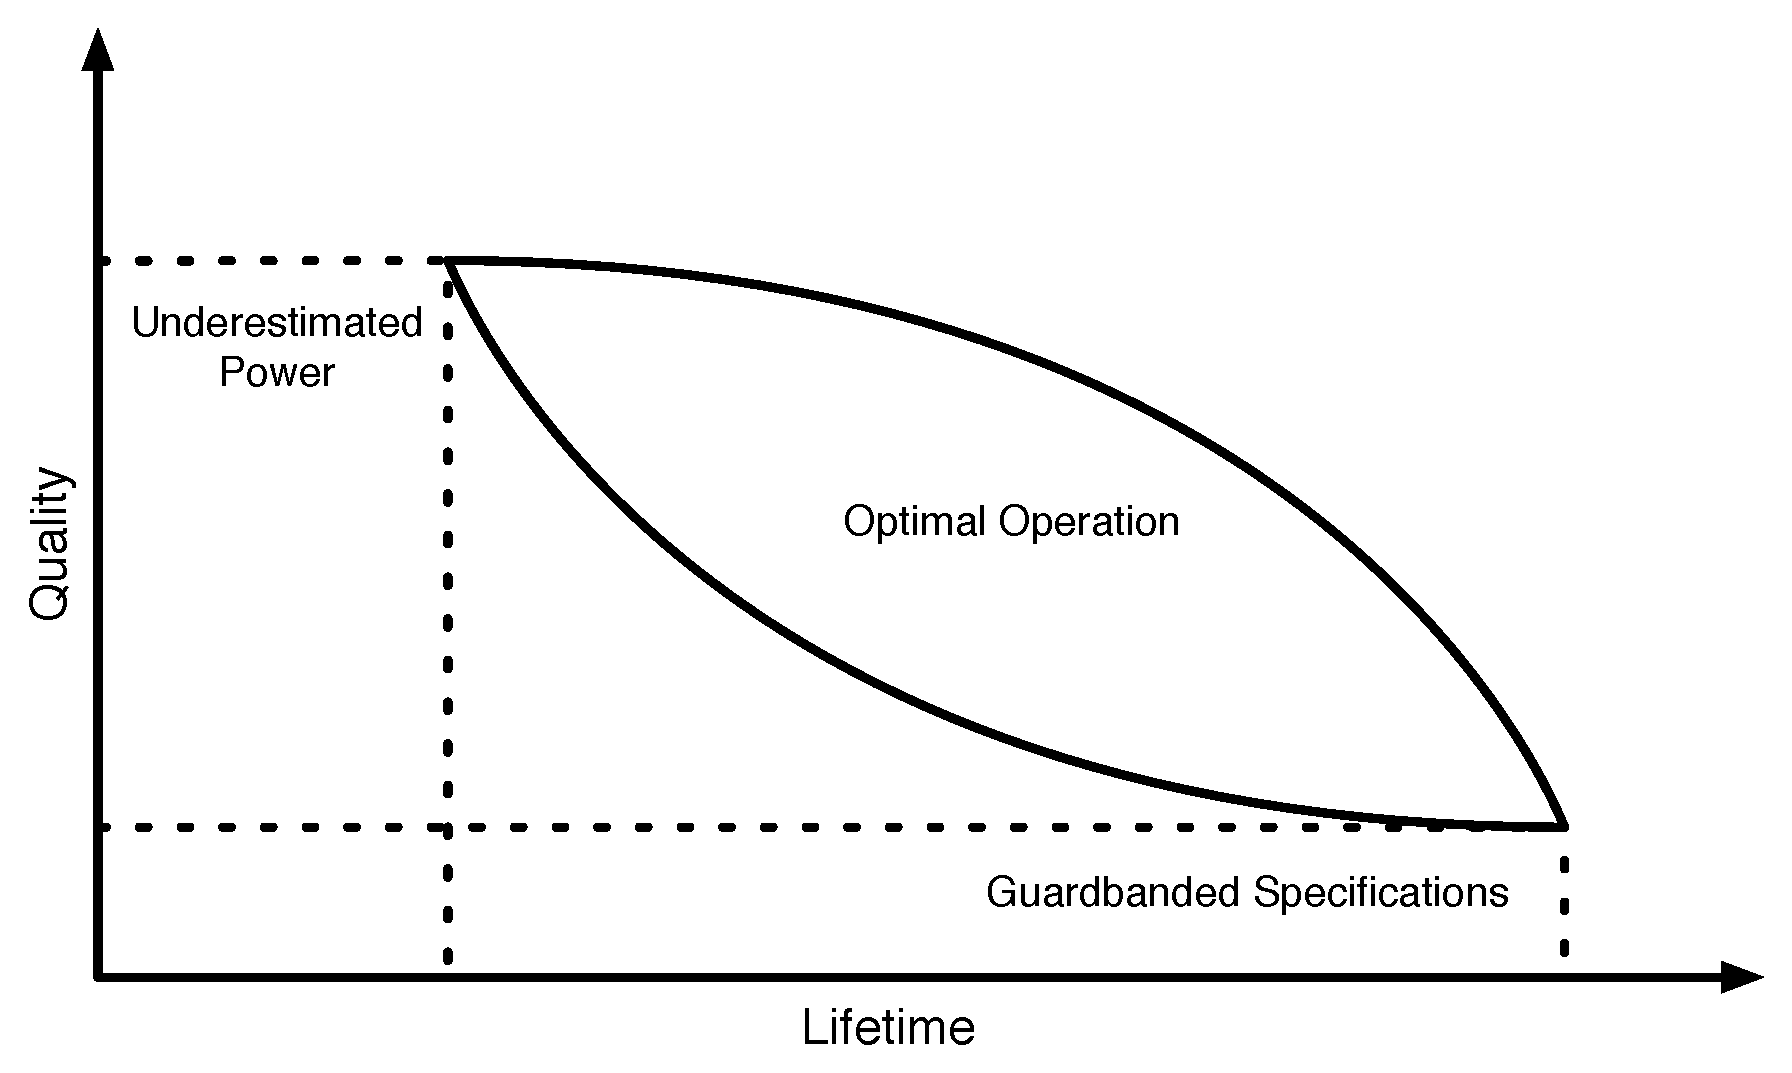
\includegraphics[width=\textwidth]{figures/intro_quality_vs_lifetime}
  \captionof{figure}{\label{fig:qualityandlifetime}potential results of variability in terms of system quality and lifetime}
\end{minipage}
}
\end{figure*}



In this work we explore the interplay between variable active and idle power consumption, deployment-specific temperature profiles, and multiple heterogeneous tasks. Specifically, we seek an answer to the question posed above; in an environment where power and temperature are measurable quantities, we seek an optimal strategy for distributing energy between arbitrary tasks in order to maximize application utility.  In answering these questions, we introduce the notion of task \emph{knobs}.  These knobs offer both a way for tasks to express elasticity in terms of utility and processing time and a way in which an operating system can fine-tune task energy consumption. Developers provide bounds on the values that each knob can assume and decide in what ways each knob is used, but optimization of these knob values is offloaded to the operating system and is done at runtime after accurate power and computational models have been constructed.  These operating system abstractions are implemented in VaRTOS, a variability-aware operating system built as an extension to an open-source embedded operating system. In order to evaluate the abstractions and architectures that make up VaRTOS, we use custom variability extensions to a popular hardware simulation suite. 

Our contributions include the following: 

\begin{itemize}
\item We develop an architecture for modeling and optimizing per-task energy consumption at the operating system level, allowing for tunable quality and, correspondingly, accurate lifetime achievement in the face of variability. 
\item We provide a tool for evaluating the effects of power variation, environmental temperature, and additional constraints on the quality of user-defined applications comprised of multiple tasks prior to system deployment.
\item We evaluate VaRTOS, a variability-aware embedded OS that requires a modest 6.8 kB of flash memory and 518 bytes of RAM
\item We evaluate the effects of VaRTOS on several prototypical case studies, using a modified version of the QEMU simulation suite \cite{qemu}.   Our results show that VaRTOS can reduce energy consumption error to below 2\% in most cases, while strategies that assume worst-case power consumption have $> 70\%$ error in many cases.
\end{itemize}


